% Projektmanagment file dropped into the project by Jones Soliman originally created by Mihael Stojkovic
% I have comment out like all the packages and things as can be seen below
% and so far only included \usepackage{longtable} in the preamble 
% as it caused compile errors
% idk if more are needed
% but i can see it's missing in the table of contents
% 'section*' has been replaced with 'subsection'

% \documentclass[a4paper,12pt]{article} ---
% \usepackage[utf8]{inputenc}
% \usepackage[T1]{fontenc}
% \usepackage[ngerman]{babel} --- [german]
% \usepackage{geometry}
% \usepackage{longtable} ---
% \usepackage{array}
% \usepackage{setspace} ---
% \usepackage{booktabs} ---
% \usepackage{hyperref} ---
% \usepackage{ragged2e} % Für bessere Textausrichtung
% \usepackage{lipsum} ---
% \usepackage{float}
% \usepackage{graphicx} % Paket für Grafiken
% \graphicspath{{bilder/}} % Pfad zum Ordner mit den Bildern
% \usepackage{tocbibind} ---

% Seitenränder anpassen
% \geometry{left=25mm, right=25mm, top=30mm, bottom=30mm}

% % Problematisches Verhalten mindern
% \sloppy % Lockert den Textumbruch
% \setlength{\emergencystretch}{3em} % Fügt mehr Flexibilität hinzu

% \title{\textbf{Projekthandbuch \\ SwarmBots}}
% \author{Version 0.3 \\ Projektleiter/in: Mihael Stojkovic \\ Projektteam: Leander Gastgeber, Jones Soliman, Arthur Burjak}
% \date{Datum: 11.01.2025}

% % \begin{document}

% \maketitle
% \tableofcontents
% \newpage
\chapter{Projekthandbuch}
\label{sec:projekthandbuch}

\section{Projektauftrag}
\initials{MS}

% \textbf{PROJEKTAUFTRAG} \\
\textbf{SwarmBots} \\
\textbf{Projektstarttermin:} 02.09.2024 \\
\textbf{Projektendtermin:} 11.04.2025 \\

\textbf{Projektziele:}
\begin{itemize}
    \item Ein Roboter, welcher eine zweidimensionale Karte der Umgebung erstellt und die anderen Roboter leitet („Guide“).
    \item Zwei „blinde“ Roboter („Tamerlan“ und „Bambi“), welche von „Guide“ geleitet werden.
    \item Einen zentralen Server zur Datenverarbeitung, -darstellung und Kommunikation zwischen den Robotern.
\end{itemize}

\textbf{Nicht-Projektziele:}
\begin{itemize}
    \item Entwicklung eines eigenen Antriebssystems für die Roboter.
    \item Bau vieler Roboter.
\end{itemize}

\textbf{Hauptaufgaben:}
\begin{itemize}
    \item Projektmanagement
    \item Software entwickeln
    \item Zusammenbau des Hauptroboters
    \item Modifikation des Hauptroboters
    \item Zusammenbau der Nebenroboter
    \item Modifikation der Nebenroboter
    \item Installation der Basisstation
\end{itemize}

\textbf{Kosten:} Ca. 400 € (zzgl. 120 € von Projektwoche 2024 (LiDAR)) \\

\textbf{ProjektauftraggeberIn:} Erich Erker \\
\textbf{ProjektleiterIn:} Mihael Stojkovic \\
\textbf{Projektteam:} Jones Soliman, Leander Gastgeber, Arthur Burjak \\

\vspace{0,5cm}
\begin{center}
\textbf{Erich Erker (ProjektauftraggeberIn) \\ Mihael Stojkovic (ProjektleiterIn)}
\end{center}

\newpage

\section{Projektzielplan}
\initials{MS}

\textbf{PROJEKTZIELEPLAN} \\

\subsection{Hauptziele}
\initials{MS}
\begin{itemize}
    \item Ein Roboter, welcher eine zweidimensionale Karte der Umgebung erstellt und die anderen Roboter leitet („Guide“), bauen.
    \item Zwei „blinde“ Roboter („Tamerlan“ und „Bambi“), welche von „Guide“ geleitet werden, bauen.
    \item Einen zentralen Server zur Datenverarbeitung, -darstellung und Kommunikation zwischen den Robotern, erstellen.
\end{itemize}

\subsection{Zusatzziele}
\initials{MS}
\begin{itemize}
    \item Balancierung der Roboter auf zwei Rädern entwickeln.
\end{itemize}

\subsection{Nicht-Ziele}
\initials{MS}
\begin{itemize}
    \item Entwicklung eines eigenen Antriebssystems für die Roboter.
    \item Bau vieler Roboter.
\end{itemize}

\newpage

\section{Projektumweltanalyse}
\initials{MS}

\begin{figure}[htbp]
    \centering
    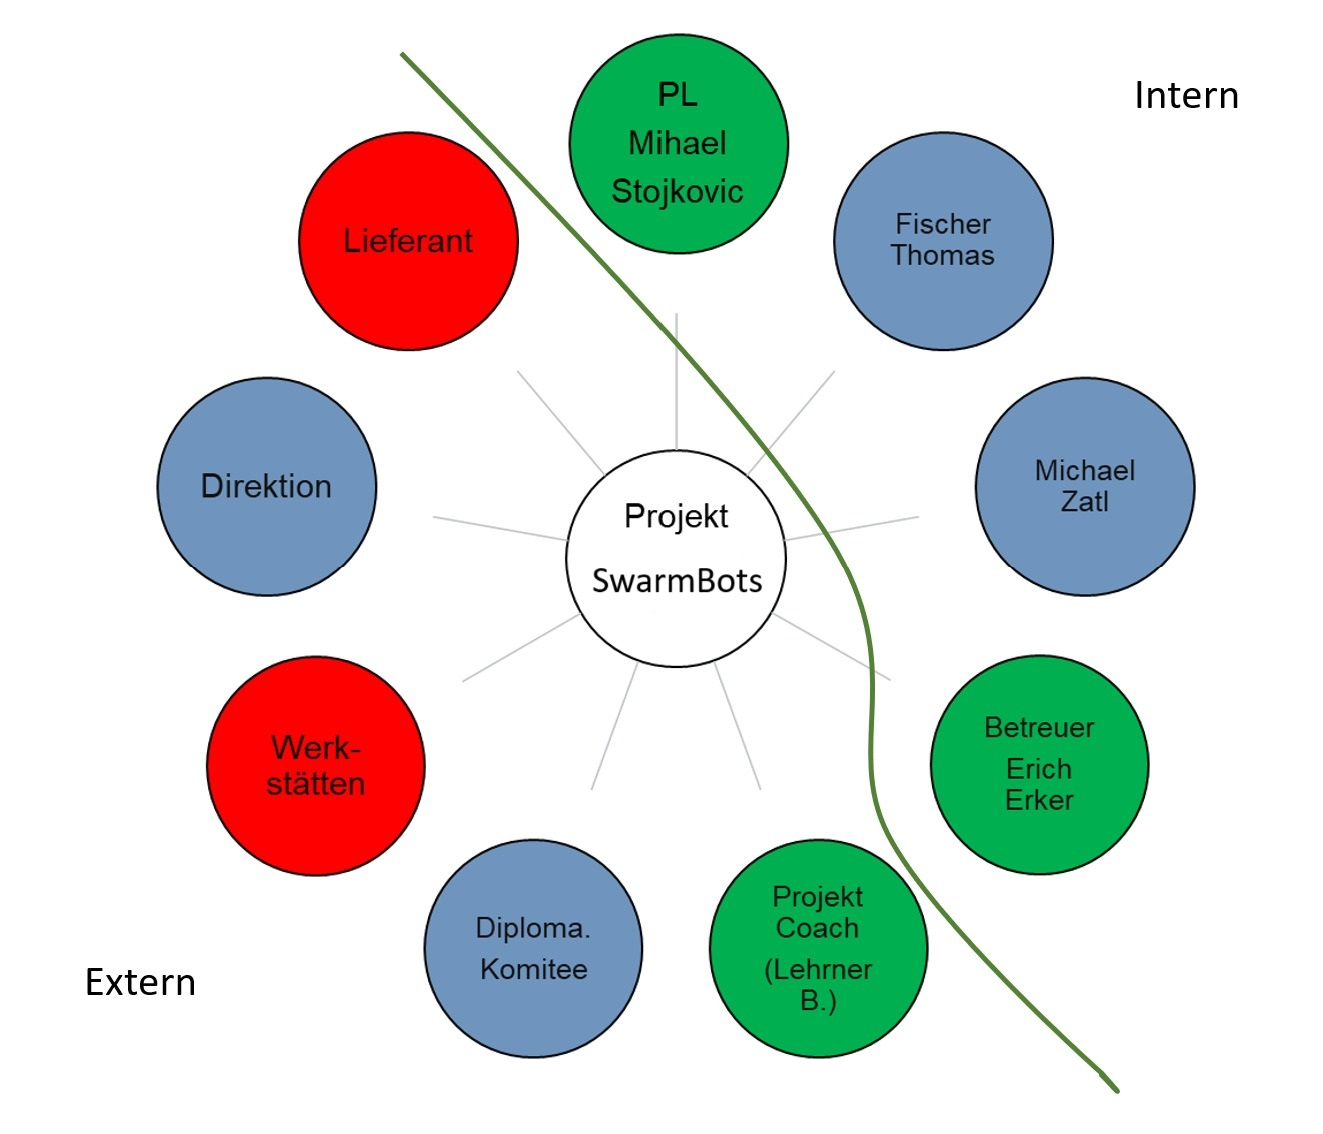
\includegraphics[width=\textwidth]{img/Projektumweltanalyse.jpeg} 
    \caption{Projektumweltanalyse}
\end{figure}

\begin{table}[H]
    \centering
    \begin{tabular}{|l|l|l|p{4.5cm}|l|}
        \hline
        \textbf{Nr.} & \textbf{P-Umwelt} & \textbf{Beziehung} & \textbf{Beschreibung} & \textbf{Maßnahmen} \\
        \hline
        1 & Lieferant & - & Evtl. Lieferverspätungen & Frühe Bestellungen \\
        \hline
        2 & Werkstätten & - & Notwendige Ressourcen evtl. nicht vorhanden & Rechtzeitige Anfragen \\
        \hline
    \end{tabular}
    \caption{Projektumwelten}
    \label{tab:projektumwelten}
\end{table}

\newpage

\section{Projektorganigramm}
\initials{MS}

\begin{figure}[H]
    \centering
    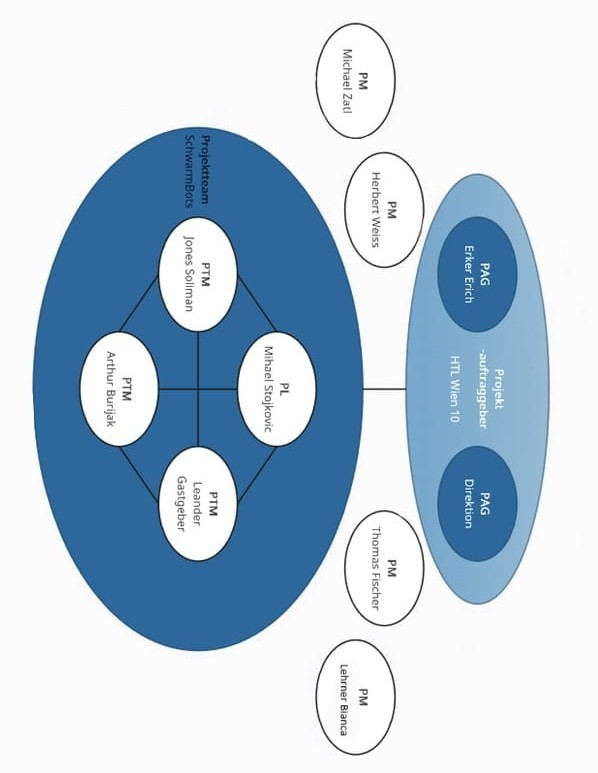
\includegraphics[width=\textwidth]{img/Projektorganigramm.jpeg}
    \caption{Projektorganigramm}
    \label{fig:organigramm}
\end{figure}


\newpage

\section{Projektobjektplan}
\initials{MS}

\begin{figure}[H]
    \centering
    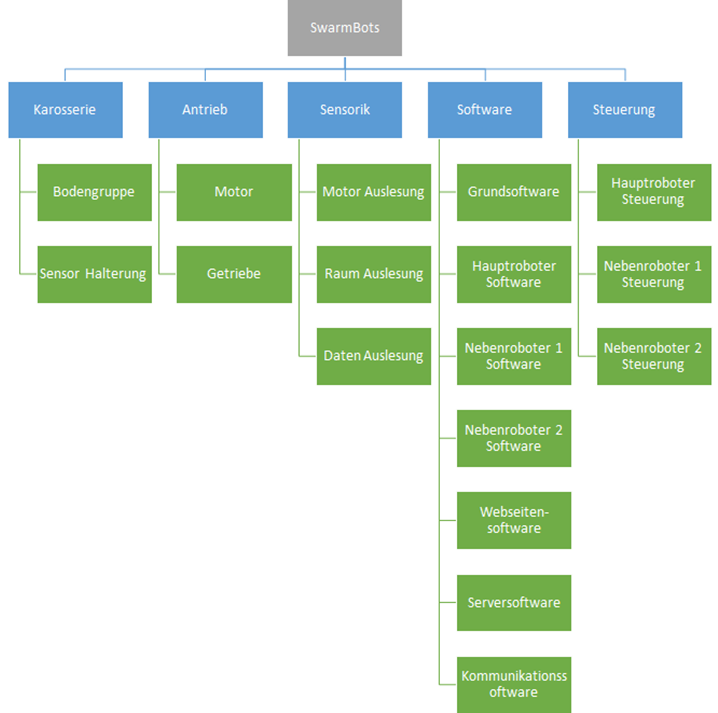
\includegraphics[width=\textwidth]{img/Projektobjektplan.png} 
    \caption{Projektobjektplan}
\end{figure}

\newpage

\section{Projektstrukturplan}
\initials{MS}

\begin{figure}[H]
    \centering
    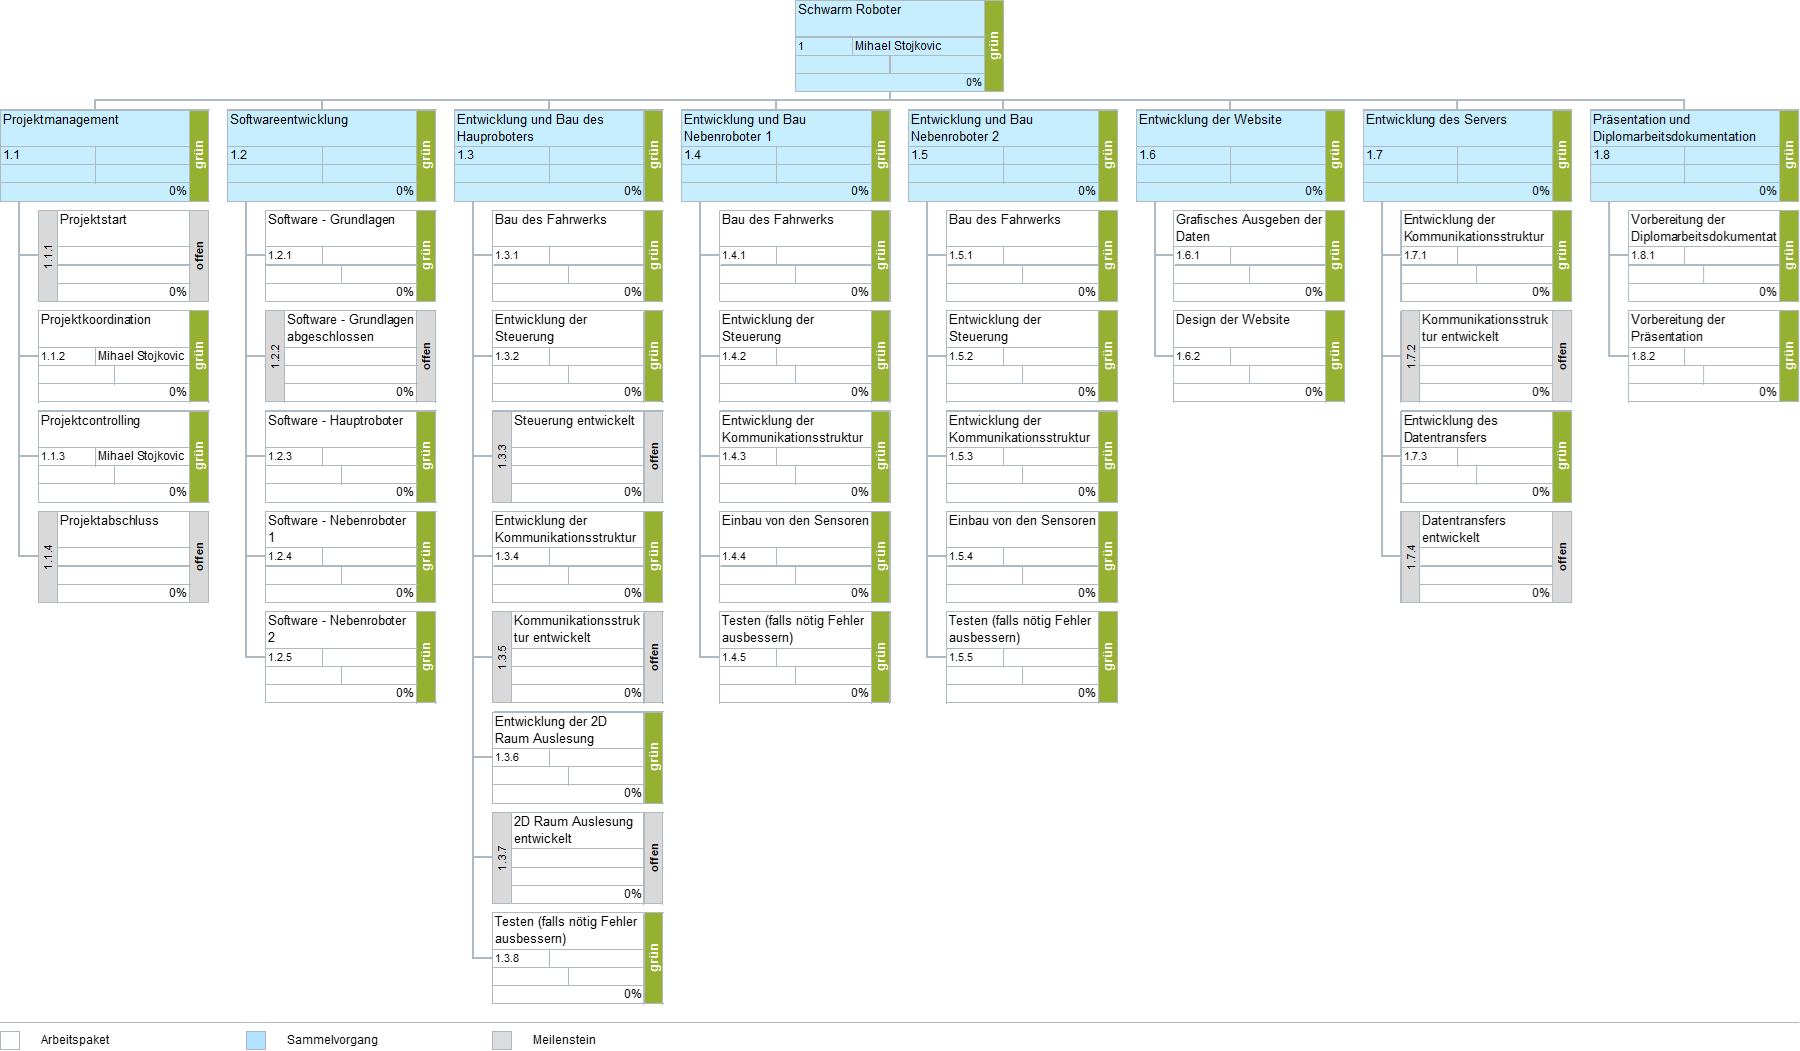
\includegraphics[width=1.4\textwidth, angle=-90]{img/Projektstrukturplan.png}
    \caption{Projektstrukturplan}
    \label{fig:psp}
\end{figure}

\newpage

\section{Projektarbeitspaketspezifikation}
\initials{MS}

\begin{longtable}[c]{|p{1cm}|p{5cm}|p{5cm}|l|}
\hline
\textbf{PSP} & \textbf{Bezeichnung} & \textbf{Inhalt} & \textbf{Verantwortlicher} \\
\hline
1.1.1 & Projektstart & Projektstart vorbereiten, Rahmenbedingungen klären, Projektplan erstellen & Mihael Stojkovic \\
\hline
1.1.2 & Projektkoordination & Aufgaben koordinieren, Fortschritt überwachen & Mihael Stojkovic \\
\hline
1.1.3 & Projektcontrolling & Zeit-, Kosten- und Ressourcenüberwachung & Mihael Stojkovic \\
\hline
1.1.4 & Projektabschluss & Abschlussbericht erstellen, Projekterfolg bewerten & Mihael Stojkovic \\
\hline
1.2.1 & Software - Grundlagen & Gemeinsame Softwarestruktur entwickeln & Leander Gastgeber \\
\hline
1.2.3 & Software - Hauptroboter & LiDAR-Software zur Umgebungserkennung entwickeln & Leander Gastgeber \\
\hline
1.2.4 & Software - Nebenroboter 1 & Sensorauslese-Software entwickeln & Jones Soliman \\
\hline
1.2.5 & Software - Nebenroboter 2 & Sensorauslese-Software entwickeln & Jones Soliman \\
\hline
1.3.1 & Bau des Fahrwerks & Fahrgestell fertigen und montieren & Mihael Stojkovic \\
\hline
1.3.2 & Entwicklung der Steuerung & Autonome Steuerung und manuelle Kontrolle entwickeln & Mihael Stojkovic \\
\hline
1.3.4 & Entwicklung der Kommunikationsstruktur & Protokolle definieren, Kommunikationswege aufbauen & Jones Soliman \\
\hline
1.3.6 & Entwicklung der 2D Raum Auslesung & LiDAR-Daten verarbeiten und vereinheitlichen & Leander Gastgeber \\
\hline
1.3.8 & Testen & Funktionalität testen, Fehler beheben & Arthur Burjak \\
\hline
1.4.1 & Bau des Fahrwerks & Fahrgestell für Nebenroboter fertigen & Mihael Stojkovic \\
\hline
1.4.2 & Entwicklung der Steuerung & Steuerungssoftware für autonomen Nebenroboter entwickeln & Mihael Stojkovic \\
\hline
1.4.3 & Entwicklung der Kommunikationsstruktur & Sensoren einbauen und Software integrieren & Arthur Burjak \\
\hline
1.4.4 & Einbau von den Sensoren & Einbau der Sensoren in den Roboter & Arthur Burjak \\
\hline
1.4.5 & Testen & Verbesserung oder Fehlerkorrektur & Arthur Burjak \\
\hline
1.5.1 & Bau des Fahrwerks & Fertigung und Bau des Fahrgestells & Mihael Stojkovic \\
\hline
1.5.2 & Entwicklung der Steuerung & Entwicklung der Software zum selbständigen Fahren und Steuern des Roboters & Mihael Stojkovic \\
\hline
1.5.3 & Entwicklung der Kommunikationsstruktur & Definition der Protokolle und Datenpakete & Jones Soliman \\
\hline
1.5.4 & Einbau von den Sensoren & Einbau der Sensoren in den Roboter & Arthur Burjak \\
\hline
1.5.5 & Testen & Verbesserung oder Fehlerkorrektur & Arthur Burjak \\
\hline
1.6.1 & Grafisches Ausgeben der Daten & Entwicklung der 2D-Karte mithilfe der LiDAR-Daten & Arthur Burjak \\
\hline
1.6.2 & Design der Website & Programmieren des Designs der Website & Mihael Stojkovic \\
\hline
1.7.1 & Entwicklung der Kommunikationsstruktur & Definition der Protokolle und Datenpakete (Server zur Website) & Jones Soliman \\
\hline
1.7.3 & Entwicklung des Datentransfers & Definition der Protokolle und Datenpakete (Server zum Roboter) & Leander Gastgeber \\
\hline
1.8.1 & Vorbereitung der Diplomarbeitsdokumentation & Unterlagen für die Dokumentation erstellen und verbessern & Arthur Burjak \\
\hline
1.8.2 & Vorbereitung der Präsentation & Präsentation vorbereiten & Arthur Burjak \\
\hline
\end{longtable}


\newpage

\section{Projektfunktionendiagramm}
\initials{MS}

\begin{longtable}[c]{|p{4,3cm}|p{1cm}|p{1cm}|p{1cm}|p{1cm}|p{1cm}|p{1cm}|p{1cm}|p{1,5cm}|}
\hline
\textbf{Arbeitspakete  /  Phasen} & \textbf{PAG (EE)} & \textbf{PL (MS)} & \textbf{PTM (LG)} & \textbf{PTM (JS)} & \textbf{PTM (AB)} & \textbf{PM (MZ)} & \textbf{PM (BL)} & \textbf{Kunde (HTL)} \\
\hline
Projektmanagement & & & & & & & & \\
\hline
Projektstart & E & D & M & M & M & I & & M \\
\hline
Projektkoordination & & D & M & M & M & I & & \\
\hline
Projektcontrolling & I & D & M & M & M & I & & M \\
\hline
Projektabschluss & M & D & M & M & M & I & & \\
\hline
Softwareentwicklung & & & & & & & & \\
\hline
Software - Grundlagen & & M & D & M & M & I & & \\
\hline
Software - Hauptroboter & & M & D & M & M & I & & \\
\hline
Software - Nebenroboter 1 & & M & D & M & M & I & & \\
\hline
Software - Nebenroboter 2 & & M & D & M & M & I & & \\
\hline
Entwicklung und Bau des Hauptroboters & & & & & & & & \\
\hline
Bau des Fahrwerks & & D & M & M & M & I & & I \\
\hline
Entwicklung der Steuerung & & M & D & M & M & I & & \\
\hline
Entwicklung der Kommunikationsstruktur & I & M & M & D & M & & I & \\
\hline
Entwicklung der 2D Raum Auslesung & & M & D & M & M & I & & \\
\hline
Testen (falls nötig Fehler ausbessern) & & D & M & M & M & & I & \\
\hline
Entwicklung und Bau Nebenroboter 1 & & & & & & & & \\
\hline
Bau des Fahrwerks & & D & M & M & M & & & I \\
\hline
Entwicklung der Steuerung & & M & D & M & M & & & \\
\hline
Entwicklung der Kommunikationsstruktur & I & M & M & D & M & & & \\
\hline
Einbau von den Sensoren & & M & D & M & M & I & & \\
\hline
Testen (falls nötig Fehler ausbessern) & & D & M & M & M & & & \\
\hline
Entwicklung und Bau Nebenroboter 2 & & & & & & & & \\
\hline
Bau des Fahrwerks & & D & M & M & M & & & I \\
\hline
Entwicklung der Steuerung & & M & D & M & M & & & \\
\hline
Entwicklung der Kommunikationsstruktur & I & M & M & D & M & & & \\
\hline
Einbau von den Sensoren & & M & D & M & M & I & & \\
\hline
Testen (falls nötig Fehler ausbessern) & & D & M & M & M & & & \\
\hline
Entwicklung der Website & & & & & & & & \\
\hline
Grafisches Ausgeben der Daten & & M & M & M & D & & & \\
\hline
Design der Website & & M & M & M & D & & & \\
\hline
Entwicklung des Servers & & & & & & & & \\
\hline
Entwicklung der Kommunikationsstruktur & I & M & M & D & M & & & \\
\hline
Kommunikationsstruktur entwickelt & I & M & M & D & M & & & \\
\hline
Entwicklung des Datentransfers & & M & M & D & M & & & \\
\hline
Präsentation und Diplomarbeitsdokumentation & & & & & & & & \\
\hline
Vorbereitung der Diplomarbeitsdokumentation & E & M & M & M & D & & & \\
\hline
Vorbereitung der Präsentation & I & M & M & M & D & & & \\
\hline
Präsentieren & E & M & M & M & D & & & \\
\hline
\end{longtable}

Legende:
\smallskip
PAG = Projektauftraggeber   |   EE = Erich Erker
PL = Projektleiter          |   MS = Mihael Stojkovic
PTM = Projektteammitglied   |   JS = Jones Soliman
PM = Projektmitglied        |   LG = Leander Gastgeber
BL = Biannca Lehrner        |   AB = Arthur Burjak  
MZ = Michael Zatl

\newpage
\section{Projektmeilensteinplan}
\initials{MS}

\begin{longtable}[c]{|p{3cm}|p{6cm}|p{3cm}|l|}
\hline
\textbf{PSP-Code} & \textbf{Meilensteinbezeichnung} & \textbf{Plantermin} & \textbf{Isttermin} \\
\hline
1.1.1 & Projektstart & 02.09.2024 & 02.09.2024 \\
\hline
1.2.2 & Software - Grundlagen abgeschlossen & 25.10.2024 & 25.10.2024 \\
\hline
1.3.3 & Steuerung entwickelt & 20.12.2024 & \\
\hline
1.3.5 & Kommunikationsstruktur entwickelt & 20.12.2024 & \\
\hline
1.3.7 & 2D Raum Auslesung entwickelt & 10.01.2025 & \\
\hline
1.7.2 & Kommunikationsstruktur entwickelt & 10.01.2025 & \\
\hline
1.7.4 & Datentransfers entwickelt & 31.01.2025 & \\
\hline
1.1.4 & Projektabschluss & 11.04.2025 & \\
\hline
\end{longtable}

\newpage

\section{Projektbalkenplan}
\initials{MS}

\begin{figure}[htbp]
    \centering
    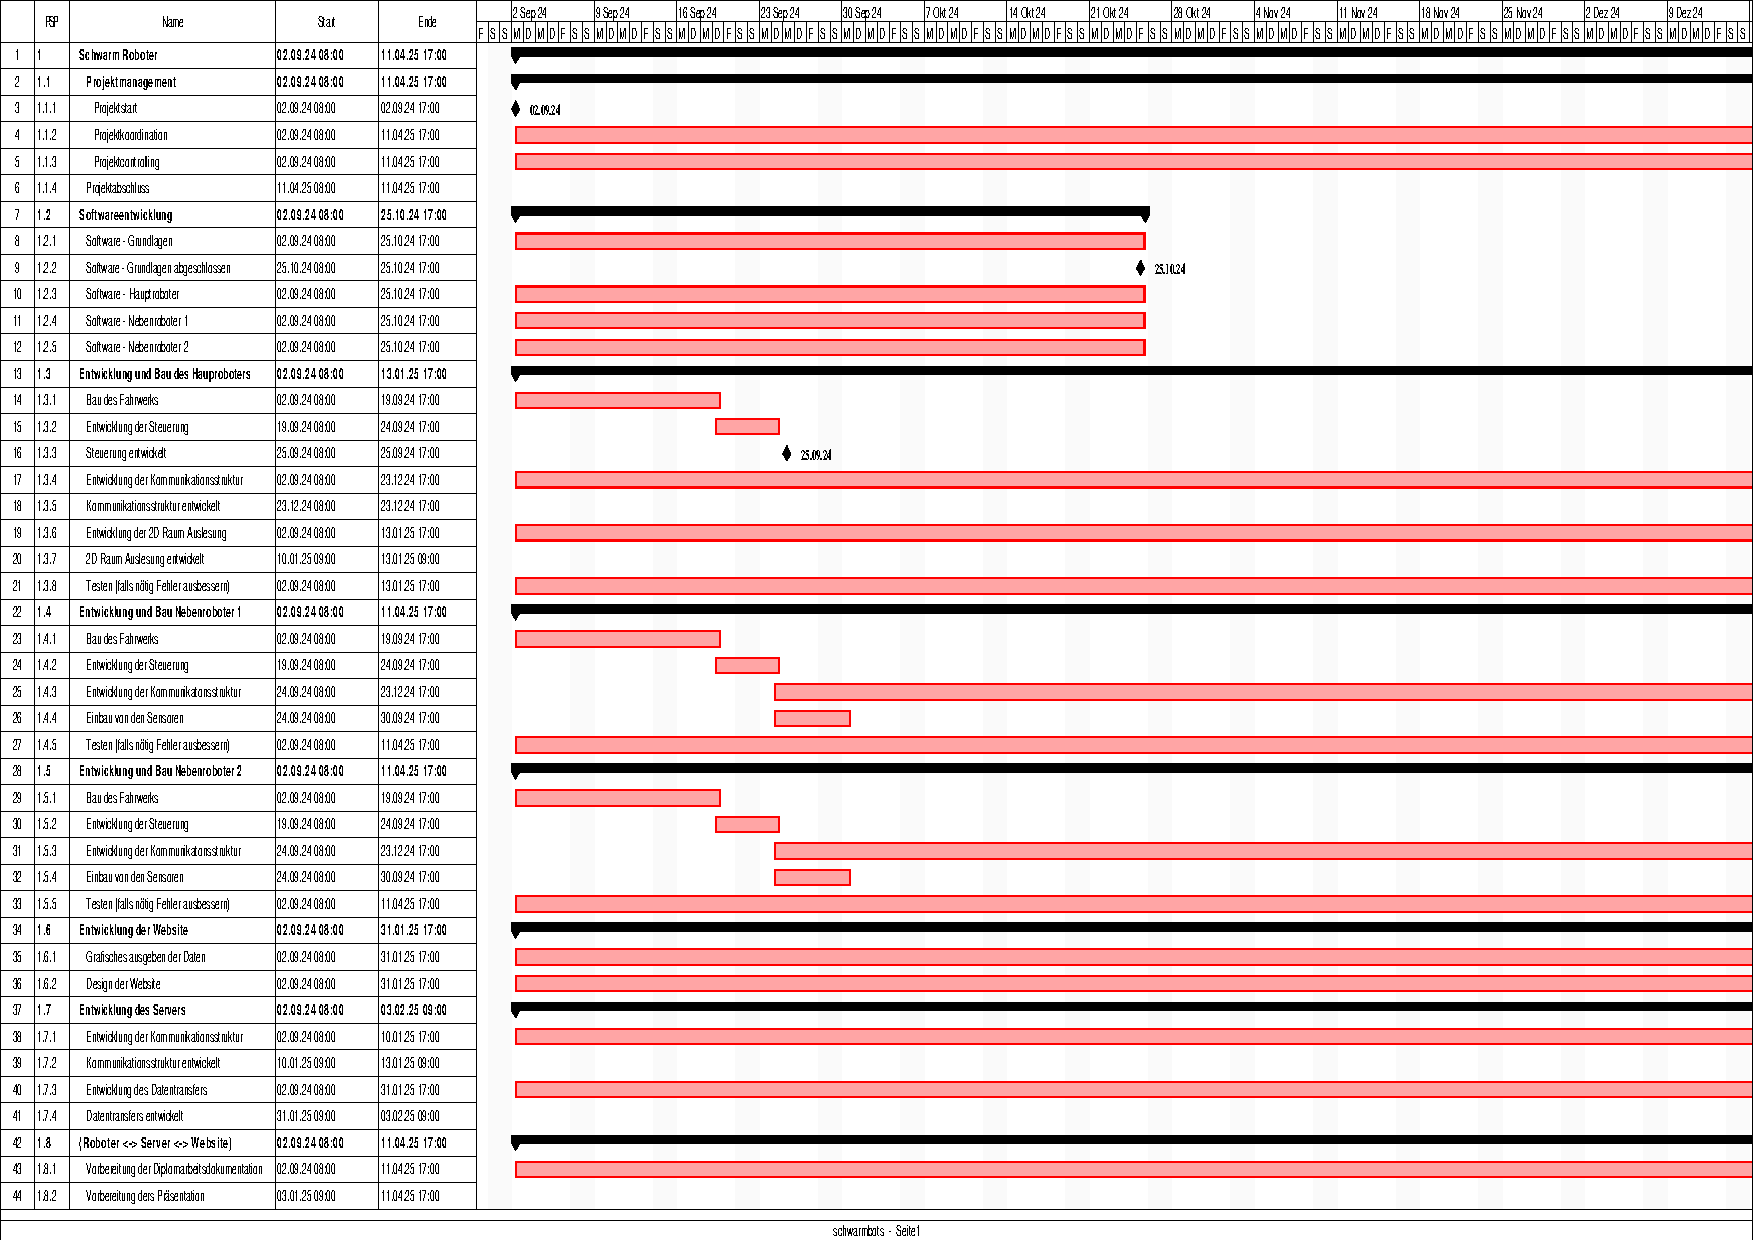
\includegraphics[width=1.18\textwidth,page=1,angle=-90]{img/Projektbalkenplan-gantt_landscape.pdf}
    \caption{Projektbalkenplan01}
    \label{fig:psp_balk}
\end{figure}
\begin{figure}[htbp]
    \centering
    \includegraphics[width=1.18\textwidth,page=2,angle=-90]{img/Projektbalkenplan-gantt_landscape.pdf}
    \caption{Projektbalkenplan02}
    \label{fig:psp_balk2}
\end{figure}
\newpage

\section{Projektkostenplan}
\initials{MS}

\begin{longtable}[c]{|p{0,8cm}|p{3cm}|p{1,9cm}|p{1,9cm}|p{2cm}|p{1,9cm}|p{1,9cm}|}
\hline
\textbf{PSP} & \textbf{Arbeitspaket} & \textbf{Personal (€)} & \textbf{Material (€)} & \textbf{Fremd-  leistung (€)} & \textbf{Sonstige (€)} & \textbf{Gesamt (€)} \\
\hline
1.1.1 & Start-Prozess & 2500 & 0 & 350 & 0 & 2850 \\
\hline
1.1.2 & Projektkoordi- nation & 2500 & 0 & 350 & 0 & 2850 \\
\hline
1.1.3 & Projektcontro- lling & 2500 & 0 & 350 & 0 & 2850 \\
\hline
1.1.4 & Projektabschluss-Prozess & 2500 & 0 & 350 & 0 & 2850 \\
\hline
1.2.1 & Software - Grundlagen & 1250 & 0 & 0 & 0 & 1250 \\
\hline
1.2.2 & Software - Grundlagen abgeschlossen & 100 & 0 & 0 & 0 & 100 \\
\hline
1.2.3 & Software - Hauptroboter & 1250 & 0 & 0 & 0 & 1250 \\
\hline
1.2.4 & Software - Nebenroboter 1 & 1250 & 0 & 0 & 0 & 1250 \\
\hline
1.2.5 & Software - Nebenroboter 2 & 1250 & 0 & 0 & 0 & 1250 \\
\hline
1.3.1 & Bau des Fahrwerks & 2250 & 90 & 0 & 0 & 2340 \\
\hline
1.3.2 & Entwicklung der Steuerung & 2500 & 0 & 0 & 0 & 2500 \\
\hline
1.3.3 & Steuerung entwickelt & 100 & 0 & 0 & 0 & 100 \\
\hline
1.3.4 & Entwicklung der Kommunikationsstruktur & 2500 & 0 & 0 & 0 & 2500 \\
\hline
1.3.5 & Kommunikations- struktur entwickelt & 100 & 0 & 0 & 0 & 100 \\
\hline
1.3.6 & Entwicklung der 2D Raum Auslesung & 1250 & 150 & 0 & 0 & 1400 \\
\hline
1.3.7 & 2D Raum Auslesung entwickelt & 100 & 0 & 0 & 0 & 100 \\
\hline
1.3.8 & Testen & 2250 & 0 & 0 & 0 & 2250 \\
\hline
1.4.1 & Bau des Fahrwerks & 2250 & 90 & 0 & 0 & 2340 \\
\hline
1.4.2 & Entwicklung der Steuerung & 2500 & 0 & 0 & 0 & 2500 \\
\hline
1.4.3 & Entwicklung der Kommunikationsstruktur & 2500 & 0 & 0 & 0 & 2500 \\
\hline
1.4.4 & Einbau von den Sensoren & 2250 & 50 & 0 & 0 & 2300 \\
\hline
1.4.5 & Testen & 2250 & 0 & 0 & 0 & 2250 \\
\hline
1.5.1 & Bau des Fahrwerks & 2250 & 90 & 0 & 0 & 2340 \\
\hline
1.5.2 & Entwicklung der Steuerung & 2500 & 0 & 0 & 0 & 2500 \\
\hline
1.5.3 & Entwicklung der Kommunikationsstruktur & 2500 & 0 & 0 & 0 & 2500 \\
\hline
1.5.4 & Einbau von den Sensoren & 2250 & 50 & 0 & 0 & 2300 \\
\hline
1.5.5 & Testen & 2250 & 0 & 0 & 0 & 2250 \\
\hline
1.6.1 & Grafisches ausgeben der Daten & 1500 & 0 & 0 & 0 & 1500 \\
\hline
1.6.2 & Design der Website & 1500 & 0 & 0 & 0 & 1500 \\
\hline
1.7.1 & Entwicklung der Kommunikationsstruktur & 1250 & 0 & 0 & 0 & 1250 \\
\hline
1.7.2 & Kommunikations-  struktur entwickelt & 100 & 0 & 0 & 0 & 100 \\
\hline
1.7.3 & Entwicklung des Datentransfers & 1250 & 0 & 0 & 0 & 1250 \\
\hline
1.7.4 & Datentransfers entwickelt & 100 & 0 & 0 & 0 & 100 \\
\hline
1.8.1 & Vorbereitung der Diplomarbeitsdokumentation & 4000 & 0 & 0 & 0 & 4000 \\
\hline
1.8.2 & Vorbereitung der Präsentation & 4000 & 0 & 0 & 0 & 4000 \\
\hline
1.8.3 & Präsentieren & 4000 & 0 & 0 & 0 & 4000 \\
\hline
\end{longtable}
%
\textbf{Zusätzliche Informationen:} \\
1.3.1 / 1.4.1 / 1.5.1: 90 € für die Roboterkits. \\
1.3.4: 150 € für den LiDAR und ESP32 Nano. \\
1.4.4 / 1.5.4: 50 € für den ESP32 Nano, ESP32 Cam und die Sensoren. \\
%
\textbf{Gesamtkosten:} 69.270 € (ohne Personalkosten: 520 €).

% \end{document}
